%% This is file FCEFyN-paper.tex is the template file for publications
%% in the "Revista de la Facultad de Ciencias Exactas, Físicas y Naturales
%% de la Universidad Nacional de Córdoba, Argentina,
%% https://revistas.unc.edu.ar/index.php/FCEFyN.
%% This file was originally written by Gustavo J. Krause.
%% First revision: 2018-07-17
%% Second revision: 2018-07-26 by Mariano Lizarraga (minor modifications)
%%
%% History:
%%           2018-07-20  First version by Gustavo Krause
%%

% Opciones específicas:
%     esp:   Idioma español (por defecto)
%     eng:   Idioma inglés
%     por:   Idioma portugués
%     blind: Se compila la versión para revisores (se ocultan datos de los autores)


\documentclass[eng]{FCEFyN-class}
%
% Título de la publicación
\title{Lakshman Rekha}

\shorttitle{Lockdown Monitoring}
       
% Autores
\author {Tanishq Goel\\ 
\normalfont Internation Institute of Information Technology\\
\normalfont Hyderabad Telangana, India\\

\href{mailto:tanishq.goel@research.iiit.ac.in}{\nolinkurl{tanishq.goel@research.iiit.ac.in}}\\}



% Datos de la publicación (serán definidas en la edición)



% Coloque aquí sus definiciones particulares
\newcommand{\vect}[1]{\mathbf{#1}}  % vectores


% Iniciar documento
\begin{document}

% Introduzca aquí el resumen en español (o en portugués si utiliza la opción [por])
\abstract{
In this paper, we aim to provide a solution that helps the institute to identify clusters of people via surveillance, and it tries to restrict the movement of residents on the campus until the situation becomes normal again. This problem is a major issue as covid cases in the campus are increasing at an alarming rate. It is clear that the second wave has reached inside the campus too. We propose a software system, that uses multiple robots, both aerial and ground to patrol the campus area and study areawise-distribution of clusters of various outdoor places at different times during the day. It can notify the person as well as the administration if someone is in close proximity to a cluster of people. It also alerts a user if he/she is found without a mask. The administration will be notified if a specific user is found to disobey rules repeatedly.
}


% Incluir título, autores, resumen, etc.
\maketitle
\thispagestyle{fancy}


% Cuerpo principal del trabajo
\section{1. Introduction}
\lettrine[findent=2pt]{\textbf{T}}{h}e COVID-19 pandemic has led to a dramatic loss of human life worldwide and presents an unprecedented challenge to public health, food systems, and the world of work. The economic and social disruption caused by the pandemic is devastating: tens of millions of people are at risk of falling into extreme poverty, while the number of undernourished people, currently estimated at nearly 690 million, could increase by up to 132 million by the end of the year.\\

Severe acute respiratory syndrome coronavirus 2 (SARS-CoV-2), which causes coronavirus disease (COVID-19), was first identified in December 2019 in Wuhan city, China, and later spread to many provinces in China.  On January 30th, 2020, the WHO declared COVID-19 a Public Health Emergency of International Concern. \\

The first SARS-CoV-2 positive case in India was reported in the state of Kerala on January 30th, 2020. Subsequently, the number of cases drastically rose. According to the press release by the Indian Council of Medical Research (ICMR) on May 8th, 2020, a total of 14,37,788 suspected samples had been sent to the National Institute of Virology (NIV), Pune, and a related testing laboratory (3). Among them, 56,342 cases tested positive for SARS-CoV-2.\\

 To impose social distancing, the “Janata curfew” (14-h lockdown) was ordered on March 22nd, 2020. A further lockdown was initiated for 21 days, starting on March 25th, 2020, and the same was extended until May 3rd, 2020, but, owing to an increasing number of positive cases, the lockdown had been extended for the third time until May 17th, 2020. \\

India recorded more than 400,000 new COVID-19 cases for the first time on Saturday as it battles a devastating second wave, and the country's massive new vaccination drive was hampered in some areas by shortages of the shots.\\
Authorities reported 401,993 new cases in the previous 24 hours, after 10 consecutive days of more than 300,000 daily cases. Deaths jumped by 3,523, taking the country's total toll to 211,853, according to the federal health ministry.\\
The surge in infections has overwhelmed hospitals, morgues and crematoriums and left families scrambling for scarce medicines and oxygen. And while India is the world's biggest producer of COVID-19 vaccines, shortages of the shots in some states hindered the opening of vaccinations for all adults.\

\subsection{1.1 Our College Scenario}
When other engineering colleges across the country were waiting for a governmental nod for resuming normalcy in academic sessions, IIITH rolled out a slew of measures as part of a pilot project that will help other technical institutes reopen their campuses with a Covid-19 readiness plan in hand. As far back as last May, when the institute provided researchers with the option of coming back to campus, protocols related to handling the pandemic were swiftly put in place. Undergraduate students too who demonstrated an inability to cope with online academic rigour for a variety of reasons were welcomed back. But now when the country is hit by the second wave of Corona, proper implementation of lockdown becomes immensely important.\hypersetup{citecolor=red}\cite{IIITH} \\

Institute has given a set of rules so as to restrict the clustering of people on the campus. However, in spite of repeated guidelines, some people still break the rules and roam and gather around in public places increasing the chance of spread of the virus. \\

This paper discusses the following ways through which the administration can remotely detect clusters or individuals disobeying the guidelines and ways by which this software provides users with a tool by which they can keep themselves safe.\\
\begin{enumerate}
    \item Using multiple ground and aerial robots and use advanced face recognition techniques to find the identity of a person.
    \item Using the study of the area-wise distribution and hence prepare a heatmap to alert an individual
    \item Using pre-installed CCTV cameras in the institute especially those near canteens where there is a high chance of gathering.
    \item It provides a map with the live location of users in it which alerts users about approaching cluster or potential risks.
\end{enumerate}


\section{2. Literature Review}
Research is extensively being done recently in the field of tracking people through facial recognition, infra-red sensors, phone tracking, etc. These researches are helping in the implementation of lockdowns, curfews, and quarantines. There are different techniques for surveillance mechanisms to detect lockdown violators. Some features like heatmap which provide users with precautionary measures are also being researched.

\subsection{2.1 Multi-Resolution Crowd Network }
In spite of the many advantages of aerial imagery for crowd monitoring and management at mass events, datasets of aerial images of crowds are still lacking in the field.
As a remedy, in this work, we introduce a novel crowd dataset, the DLR Aerial Crowd
Dataset (DLR-ACD), which is composed of 33 large aerial images acquired from 16
flight campaigns over mass events with 226,291 persons annotated. To the best of our
knowledge, DLR-ACD is the first aerial crowd dataset and will be released publicly. The results demonstrate that MRCNet outperforms the state-of-the-art crowd counting methods in estimating the crowd counts and density maps for both aerial and CCTV-based images.\\

This mechanism uses an encoder-decoder structure to extract image features and generate crowd density maps.. It takes a single image of arbitrary
size and, in a fully convolutional manner, predicts two density maps, one with 1/4 of the
input image size for the people counting task and the other one with the input image size for
the density map estimation task. For the encoder, MRCNet relies on a pre-trained VGG-16
network [19] (without batch normalization) composed of five CNN blocks, where the spatial
size is reduced by half after each block using a max-pooling layer. The decoder is composed
of five CNN blocks, each preceded by an up-sampling layer based on bilinear interpolation
which increases the spatial size by a factor of two. \hypersetup{citecolor=red}\cite{MRC}\\

This technique can be utilized in addition to high-tech drones and robots. This technique is shown to have better results when compared to the conservative ways of aerial and ground imagery.
This technique could be also utilized for mass events spread over wide-open areas with thousands of people attending. Due to advances in airborne technology.

\subsection{2.2 Facenet}
The importance of facial recognition is known worldwide and its use is widespread but certain AI aficionados feel the need to regulate its use due to privacy issues. 
Certain malpractices can be done with the help of facial recognition like data leakage so this system should be utilized carefully .after all the drawbacks it is still the most used system. 
A facial recognition software called Facenet uses a deep Convolutional technique to attain accuracy in recognition, verification, and clustering .\\

 In this paper, we utilized a system, called FaceNet, that directly learns a mapping from face images to a compact Euclidean space where distances directly correspond to a measure of face similarity. Once this space has been produced, tasks such as face recognition, verification, and clustering can be easily implemented using standard techniques with FaceNet embeddings as feature vectors.
 The benefit of our approach is much greater representational efficiency: we achieve state-of-the-art face recognition performance using only 128-bytes per face. \cite{Facenet}\\

According to Reuter’s china used this technique to track a person from Hangzhou who was supposed to be in quarantine. Despite the fact he was wearing the mask, he was identified accurately and hence the questions about the mask being a hindrance were resolved. Hanwang technology developed two products with the help of 20 research team staff called the single Channel for entrances and multi-channel which involved many surveillance cameras. The system showed an accuracy of recognizing 95per cent people with masks and 99.5percent without masks.  Russian city like Moscow has also adopted this system with the help of smartphone apps to be able to monitor infected individuals by officials. \\

This system could be merged with the advanced tech robots and drones we have so that these algorithms could be run on the footage and we could ID the persons without actually involving any human personnel. Implementation of this algorithm is obviously not possible on a world level but at a campus level, it still seems possible.

\subsection{2.3  A real-time DNN-based face mask detection system }
Face Mask detection has turned up to be an astonishing problem in the domain of image processing and computer vision. Face detection has various use cases ranging from face recognition to capturing facial motions, where the latter calls for the face to be revealed with very high precision.

A major concern for the authorities is that residents sometimes disobey lockdown rules like by not wearing masks so we implement this system alongside our facial recognition. By this, aerial and ground machinery will help us in figuring out if a resident is roaming without a mask so that he can be alerted. Below is a brief introduction to the algorithm.\\

\begin{figure}[!htb]
 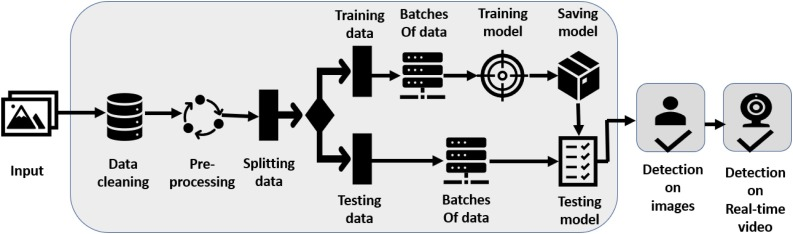
\includegraphics[scale=2]{filesFCEFyN-class/gr1_lrg.jpg} 
 \caption{Flow Diagram of the DNNV model.} 
 \label{fig-2}
\end{figure}

\subsection{2.3 Smart technologies driven approaches to tackle COVID-19 pandemic}
The implementation of new innovations and novel tactics has proven to be effective in curbing the risk of COVID-19. The present study covers the role of smart technology in mitigating the spread of COVID-19 with a specific focus on advancement in the field of drone, robotics, artificial intelligence (AI), mask, and sensor technology.\\ 

The findings shed light on the robotics and drone technology-driven approaches that have been applied for assisting health systems, surveillance, and disinfection process, etc. The AI technology strategies and framework are highlighted in terms of bulk data computing, predicting infection threats, providing medical assistance, and analyzing diagnosis results.\hypersetup{citecolor=red}\cite{Smart}\\

As we live in a time where technology is advancing rapidly, we should try to utilize it for our benefit. Here, in this paper stats were analyzed about how these machines reduce the need for human personnel and also high-tech robots make it possible to patrol the whole campus easily which would not have been possible humanely.


\begin{figure}
 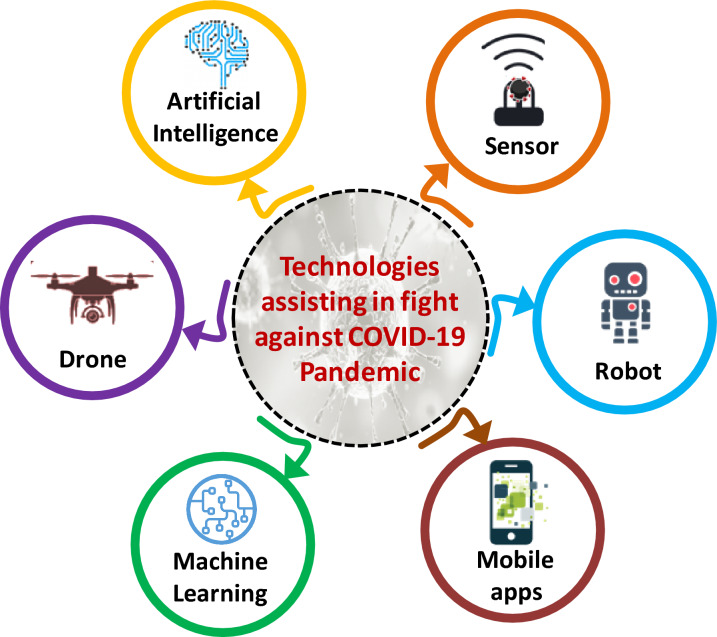
\includegraphics[scale=0.4]{filesFCEFyN-class/pic12.jpg} 
 \caption{Schematic showing smart-tech assisting in implementing lockdown} \label{fig-2}
\FloatBarrier
\end{figure}

\section{3. System Architecture}

Here, we propose a novel system that combines the above-mentioned measures and tries to restrict the unnecessary movement of residents. Since a single system cannot work everywhere, the system proposed
is designed such as to show the aspect of adaptability.

\subsection{3.1 Users}
There are two main types of users in this system
\begin{enumerate}
\item Residents: the ordinary people who are supposed to stay at home, unless they have a proper reason to leave their homes: essential groceries, immediate healthcare, essential workers, etc.

\item Administration: Who monitors the system to find those residents who break the rules.
\end{enumerate}


\subsection{3.2 Workflow}
\begin{enumerate}
\item  It is required for all the residents on the campus to create an account in the web app. It uses an AADHAR number for verification. AADHAR is kept as the sole validator as we have tried to not link this app through the college database for privacy reasons. At least 10-15 photos would be needed while registration from different angles for facial recognition purposes. 

\item After validation, residents would be given a hand band that tracks the location of a person and also keeps track of the reasons for breaching the lockdown. It also alerts the user if he is approached by a cluster of people.

\item A proper portal for reasons will be there in the application and all the residents need to apply for permission with proper reasons and corresponding time spans. The administrator validates the reason and if found genuine, the application is approved. However, in case of an emergency (like a medical emergency), the person can mention that it is an emergency.
\item Once a person is out of the hostel/ home, he/she can be tracked by the admins with the use of mechanical robots(both ground and aerial). Also, it is mandatory for each resident to keep the mask on during the time span of their stay outside their home.
\item Through different available devices(CCTV, drones, ground robots, hand band tracker), admins can track the movement and could easily find clusters of people who are roaming without masks.

\item If a person comes in the frame of video sent by the devices to the server, facial recognition algorithms are run and the ID of the person is identified. If the person breaches any of the lockdown rules, the administration office is notified and they can take the necessary action.

\item If a person cannot be identified but it can be made certain that the person is breaching some of the rules, then the person can be identified by calling ground robots at the person's position to get a clearer picture of the offender. A hand band tracker would also come in handy in those situations.

\end{enumerate}
\begin{figure}[!htb]
 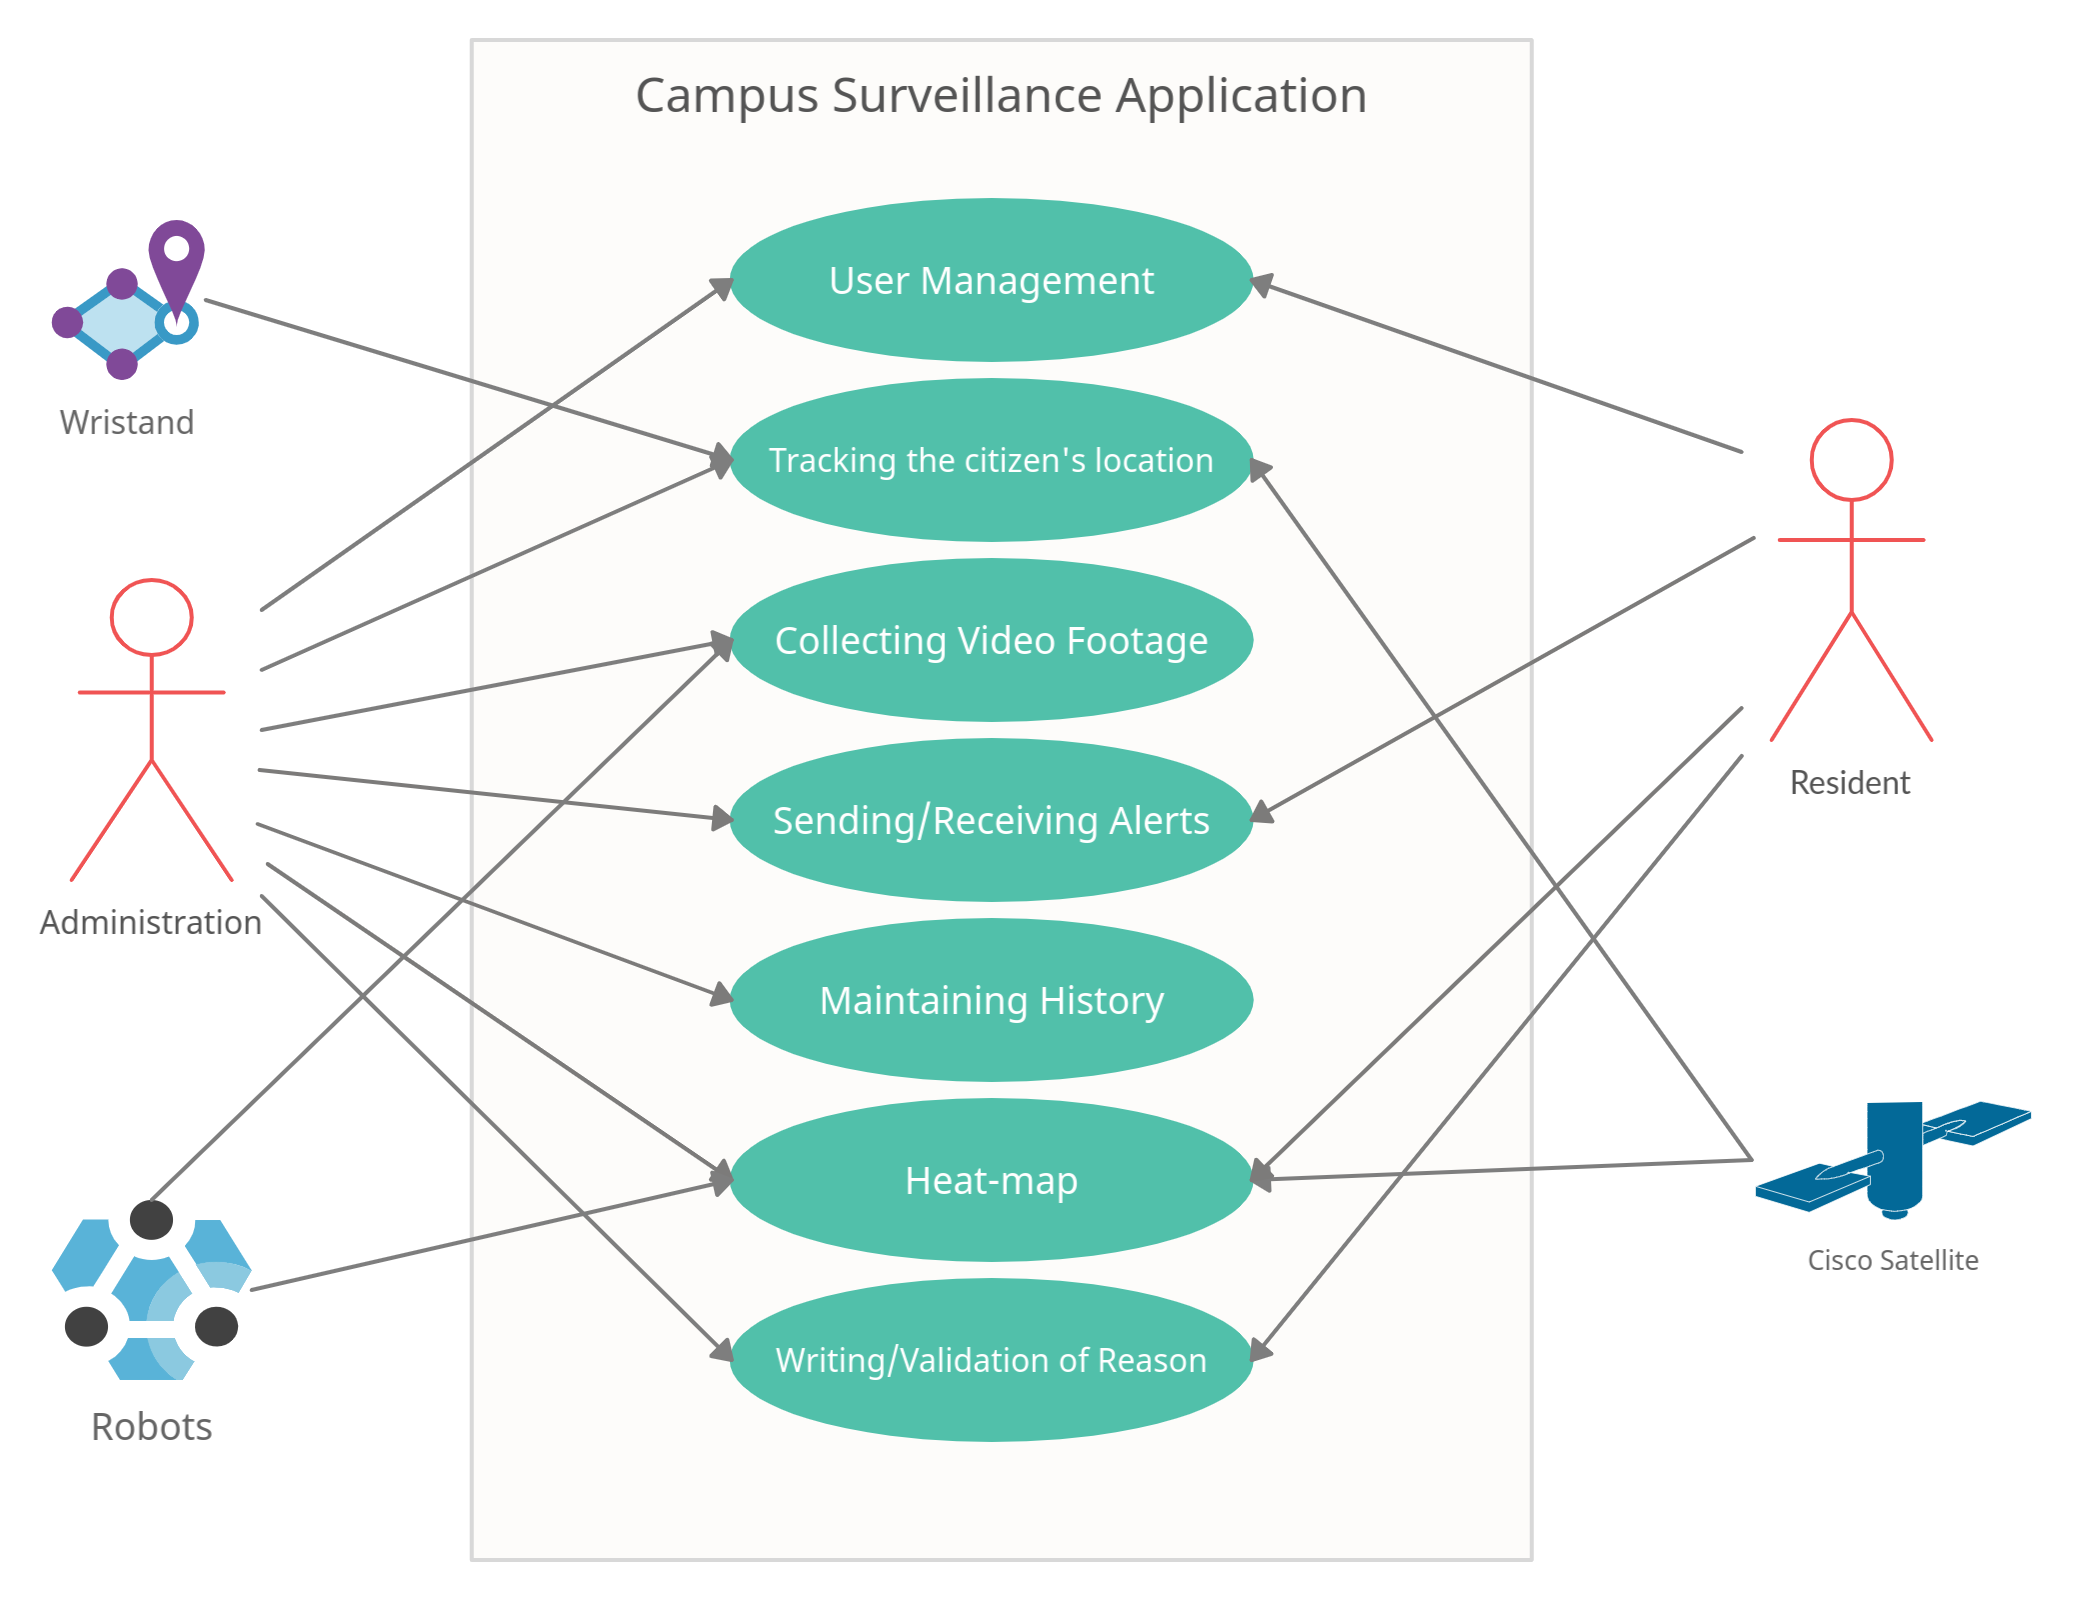
\includegraphics[scale=0.12]{filesFCEFyN-class/usecase.png} 
 \caption{UML Use Case Diagram} \label{fig-2}
 \FloatBarrier
\end{figure}

\subsection{3.3 Requirements}
The various requirements of this application can be drawn in a Use Case Diagram as in figure 1 :
\subsubsection{3.3.1 Functional Requirements}
\begin{enumerate}
    \item \textbf{User Management}: A safe and secure portal is required for the registration of accounts and also to handle logins/logouts. This portal should be able to access the government database for validation by AADHAR number.
    
    \item \textbf{Delivery of hand band}: All the users after registering in the web app will be needed to pass the manual validation as well. After manual validation, all the users would be provided with a hand band with a tracking chip and all the privacy-related concerns would be cleared out then only.\\
    \item \textbf{Application}: An application would be developed to take care of the reasons listed by the reasons with time span for which they breached/ will be breaching the lockdown. This portal will also allow admins to validate or reject the applications accordingly.
    
    \item \textbf{Tracking}: Hand Band or some other kind of tracking chip would be used to track a person's location as discussed above. This will allow admins to find a hotspot of clustering of students/staff.
    
    \item \textbf{Storing of Footage}: High tech robots will be required for both aerial and ground patrols. Video footage will be sent to the server where frames will be passed through facial recognition. If no person is identified, then that footage would be scrapped to reduce the amount of garbage data. 
    
    \item \textbf{Alerts}: Admins will have the option to send alerts to lockdown breacher and repeated alerts might lead to a warning and issue will be raised to higher authorities in case of reaching the limit of warnings.
    \item \textbf{History}: Each user and admins can view the list of reasons, applications, alerts history. Necessary features in the portal will be implemented.
\end{enumerate}

\subsubsection{3.3.2 Non-Functional Requirements}
\begin{enumerate}
    \item \textbf{Security}: The data regarding the location of a resident on the campus or footage of live recordings will be available only and only to the administration office. Necessary features would be implemented so that data could not be shared outside the application under any circumstances. All privacy-related issues would be taken care of.
    
    \item \textbf{Malfunctioning of Hand band chip}: Portal would also have a section for the maintenance of these bands. These bands will also have a feature that will signify whether the person is carrying the band or not. 
    
\end{enumerate}
\begin{figure*}
    \centering
    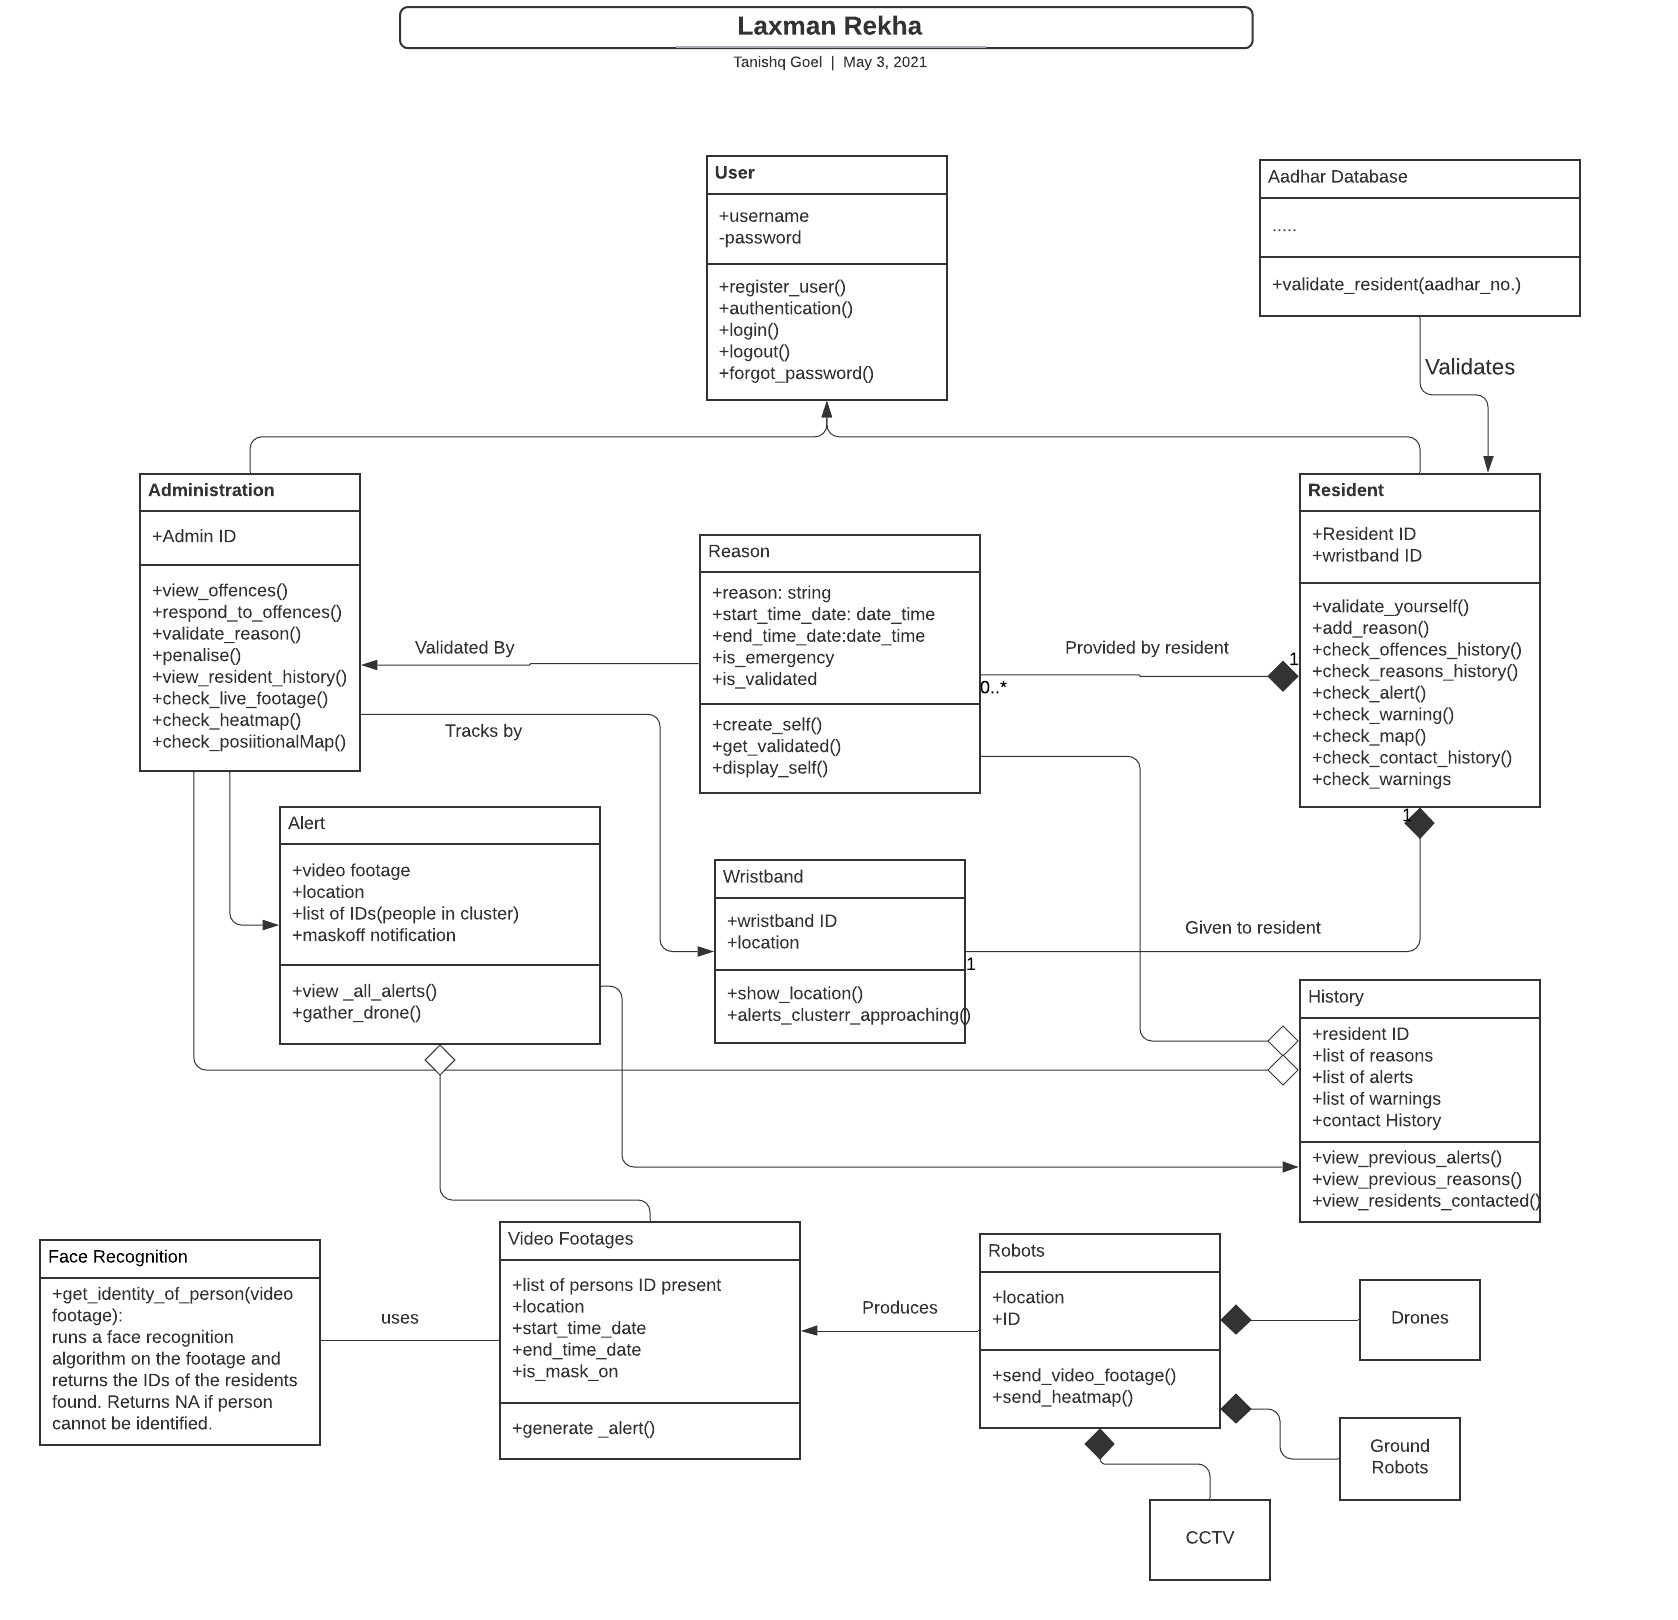
\includegraphics[scale= 0.7]{filesFCEFyN-class/Laxman_Rekha.png}
    \caption{UML Class Diagram}
    \label{fig:my_label}
    \FloatBarrier
\end{figure*}
\subsection{3.4 Classes}
\begin{enumerate}
    \item \textbf{User}: A class of user exists with basic variables including username and password with methods like registration, login, logout, etc. Users can be of two types: Admins and Residents
    \item \textbf{Administrator}: This class is the primary user of the application as an admin monitors the app. He has access to live footage recordings and locations of people who are not in their hostels or home. He sends alerts to the users if a rule is breached.
    \item \textbf{Resident}: Resident can apply for permissions to go out by providing necessary reasons. He can also see his/her history of reasons, alerts, and contacts, etc. He is also provided access to a heat map which can caution the user if a potential threat is there like the incoming of a cluster or a person without a mask.
    
    \item \textbf{AADHAR Database}: This class consists of just methods to extract AADHAR numbers from the government database.
    \item \textbf{HandBand ID}: This class consists of Hand Band ids and their respective location. This class is used by admins to track the locations of the users.
    \item \textbf{Video Footage}: This class gathers its data from the use of high-tech machines like drones. It sends footage to the server of the office.
    \item \textbf{Robot}: This class consists of drones, pre-installed CCTV ground robots which are its subclass. These classes have methods that transfer the live footage to the server room where the video clips are passed through numerous algorithms and stored if found necessary.
    \item \textbf{Face Recognition}: For the sake of this paper, this algorithm is considered as a black box that returns the ID of the residents by analyzing the video clips. If it fails to identify the person, it returns NA.
    \item \textbf{Alert}: This class consists of the rule that was breached issued by the admin office. Each alert is checked manually by the admin office and action is taken if deemed necessary.
    \item \textbf{History}: This class consists of a proper history of certain aspects of the application like alerts, reasons, and warnings.
\end{enumerate}


\subsection{3.5 Features}
\begin{enumerate}
    \item \textbf{High-tech robots}: We will be utilizing multiple robots to implement this software. Drones will be used for aerial imagery as well as to provide heat maps of a given area. Clusters of people could be identified by studying the area-wise distribution data. Hand Band contains a tracking chip that helps the administration office to track down a person. This feature can be utilized in numerous cases like in cases when the face recognition system fails to identify a person. In those situations, the person could be identified by zeroing out the location on the basis of this device.

    Our software also consists of ground robots that patrol all over the campus, even in places where drones fail to operate due to lack of signal at certain places. All the robots will be equipped with high-resolution cameras which supplements the face recognition algorithm.
    
    \item \textbf{Multi-Resolution Crowd Network}: A dataset of a high number of high-quality pictures will be collected with the help of drones and then this algorithm of multi-resolution crowd network will be applied. The dataset will be studied and analyzed thoroughly to identify hotspot areas. 
    
    \item \textbf{HeatMap by Drone Shot}: Thermal Imaging sensors are commonly referred to in terminology such as thermal camera, temperature camera, heat vision camera, infrared camera, heat signature camera, and even thermal heat vision sensor. In this post, we will refer to this type of imaging as infrared or thermal imaging. All objects (above absolute zero) emit infrared energy as a function of their temperature. Infrared energy is generated by the vibration of atoms and molecules. 
    
    \item \textbf{Portal}: A safe and secure portal that handles all the methods mentioned above in the UML Class diagram. Its use ranges from user management to Heat-map display which can be highly beneficial for the user.

    \begin{figure}[!htb]
        \centering
        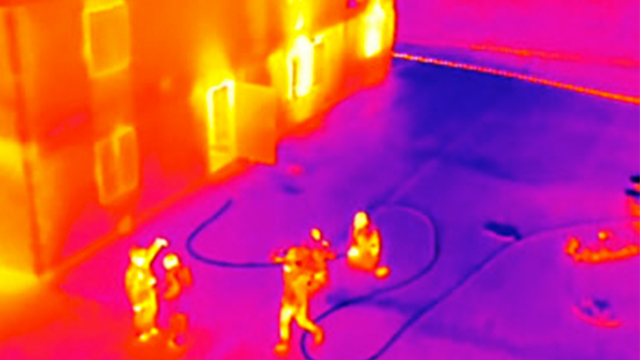
\includegraphics[scale =0.4]{filesFCEFyN-class/infra.jpg}
        \caption{HeatMap by Drone shot}
        \label{fig:my_label}
        \FloatBarrier
    \end{figure}
\end{enumerate}
\subsection{3.6 Sequence Diagram}
Fig 6 and Fig 7 shows two sequence diagrams for features implemented which are login and request for innocence respectively.
\vspace{1.3cm}
\begin{figure}[!htb]
 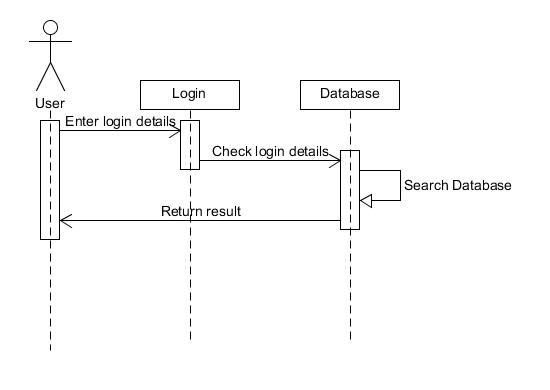
\includegraphics[scale=0.4]{filesFCEFyN-class/login_sd.jpg} 
 \caption{Login Sequence Diagram} \label{fig-2}
 \FloatBarrier
\end{figure}

\begin{figure}[!htb]
 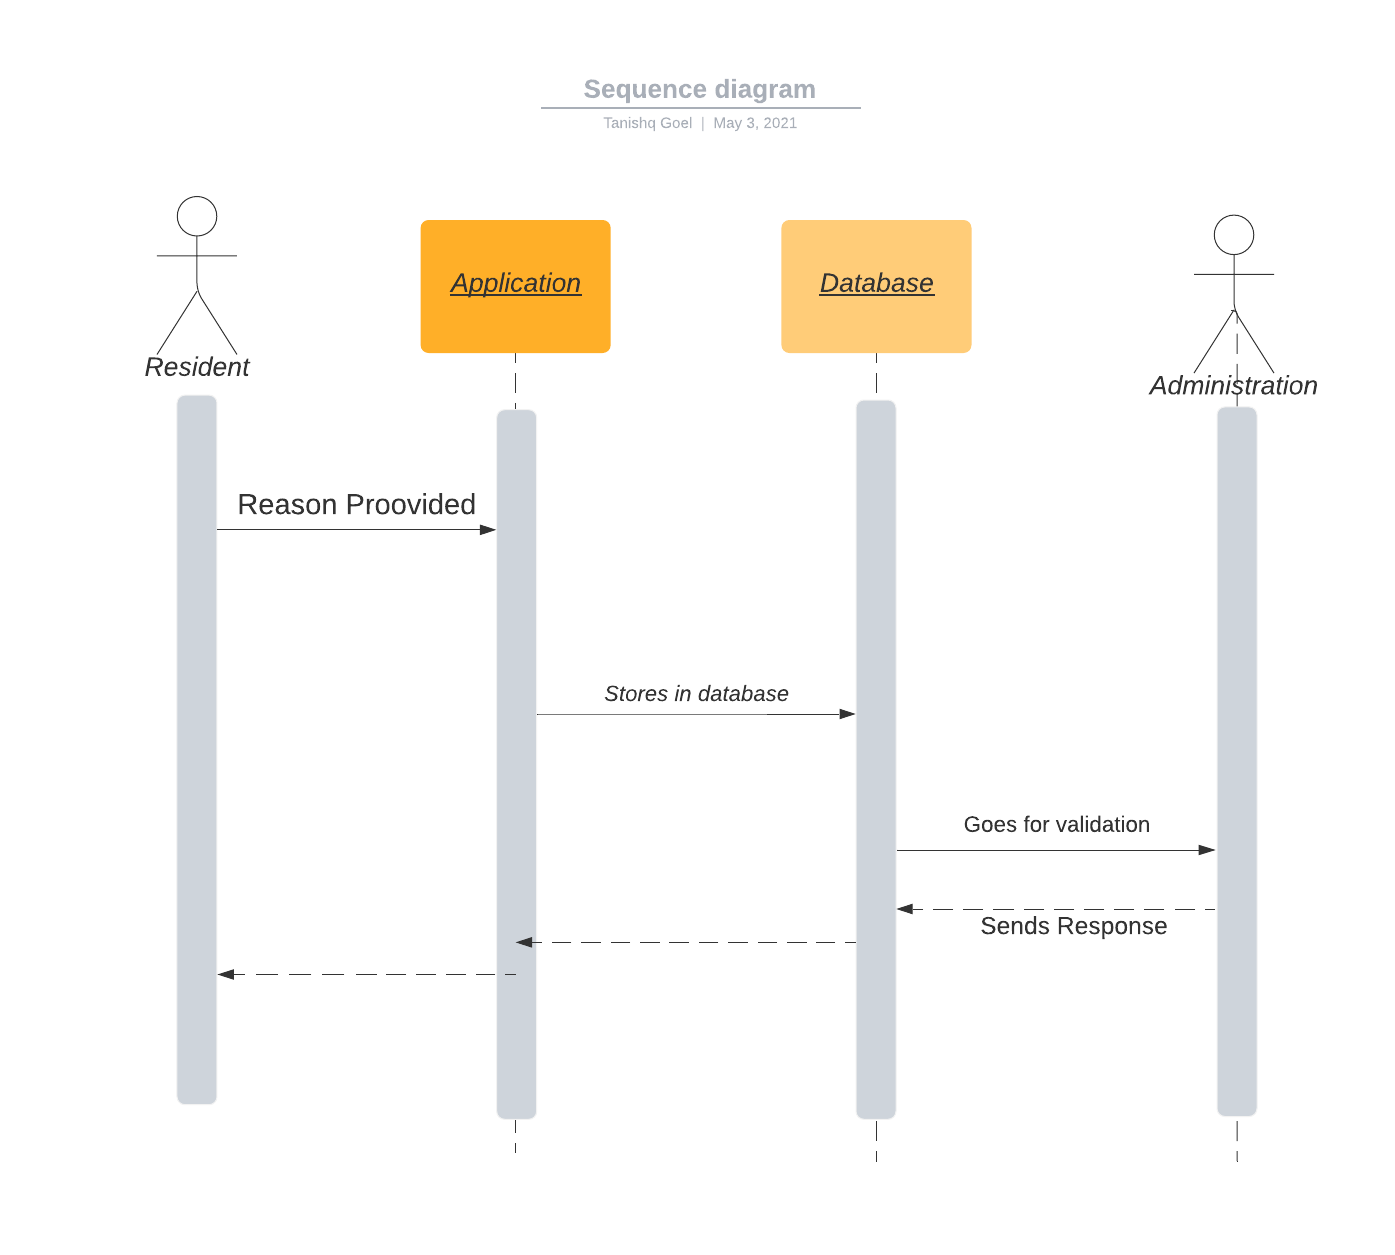
\includegraphics[scale=0.35]{filesFCEFyN-class/drone_sd.png} 
 \caption{Reason Application Sequence Diagram} \label{fig-2}
 \FloatBarrier
\end{figure}

\subsection{3.7 State Diagram}
Fig 8 shows the state diagram for the software. The process begins when video devices record the videos and send them to the server office. Then multiple algorithms are run to analyze and ID the person. If a resident is found to breach any rule, an alert is issued to the resident. Necessary actions are taken by the authorities from the output received from the algorithms.
\begin{figure}[!htb]
 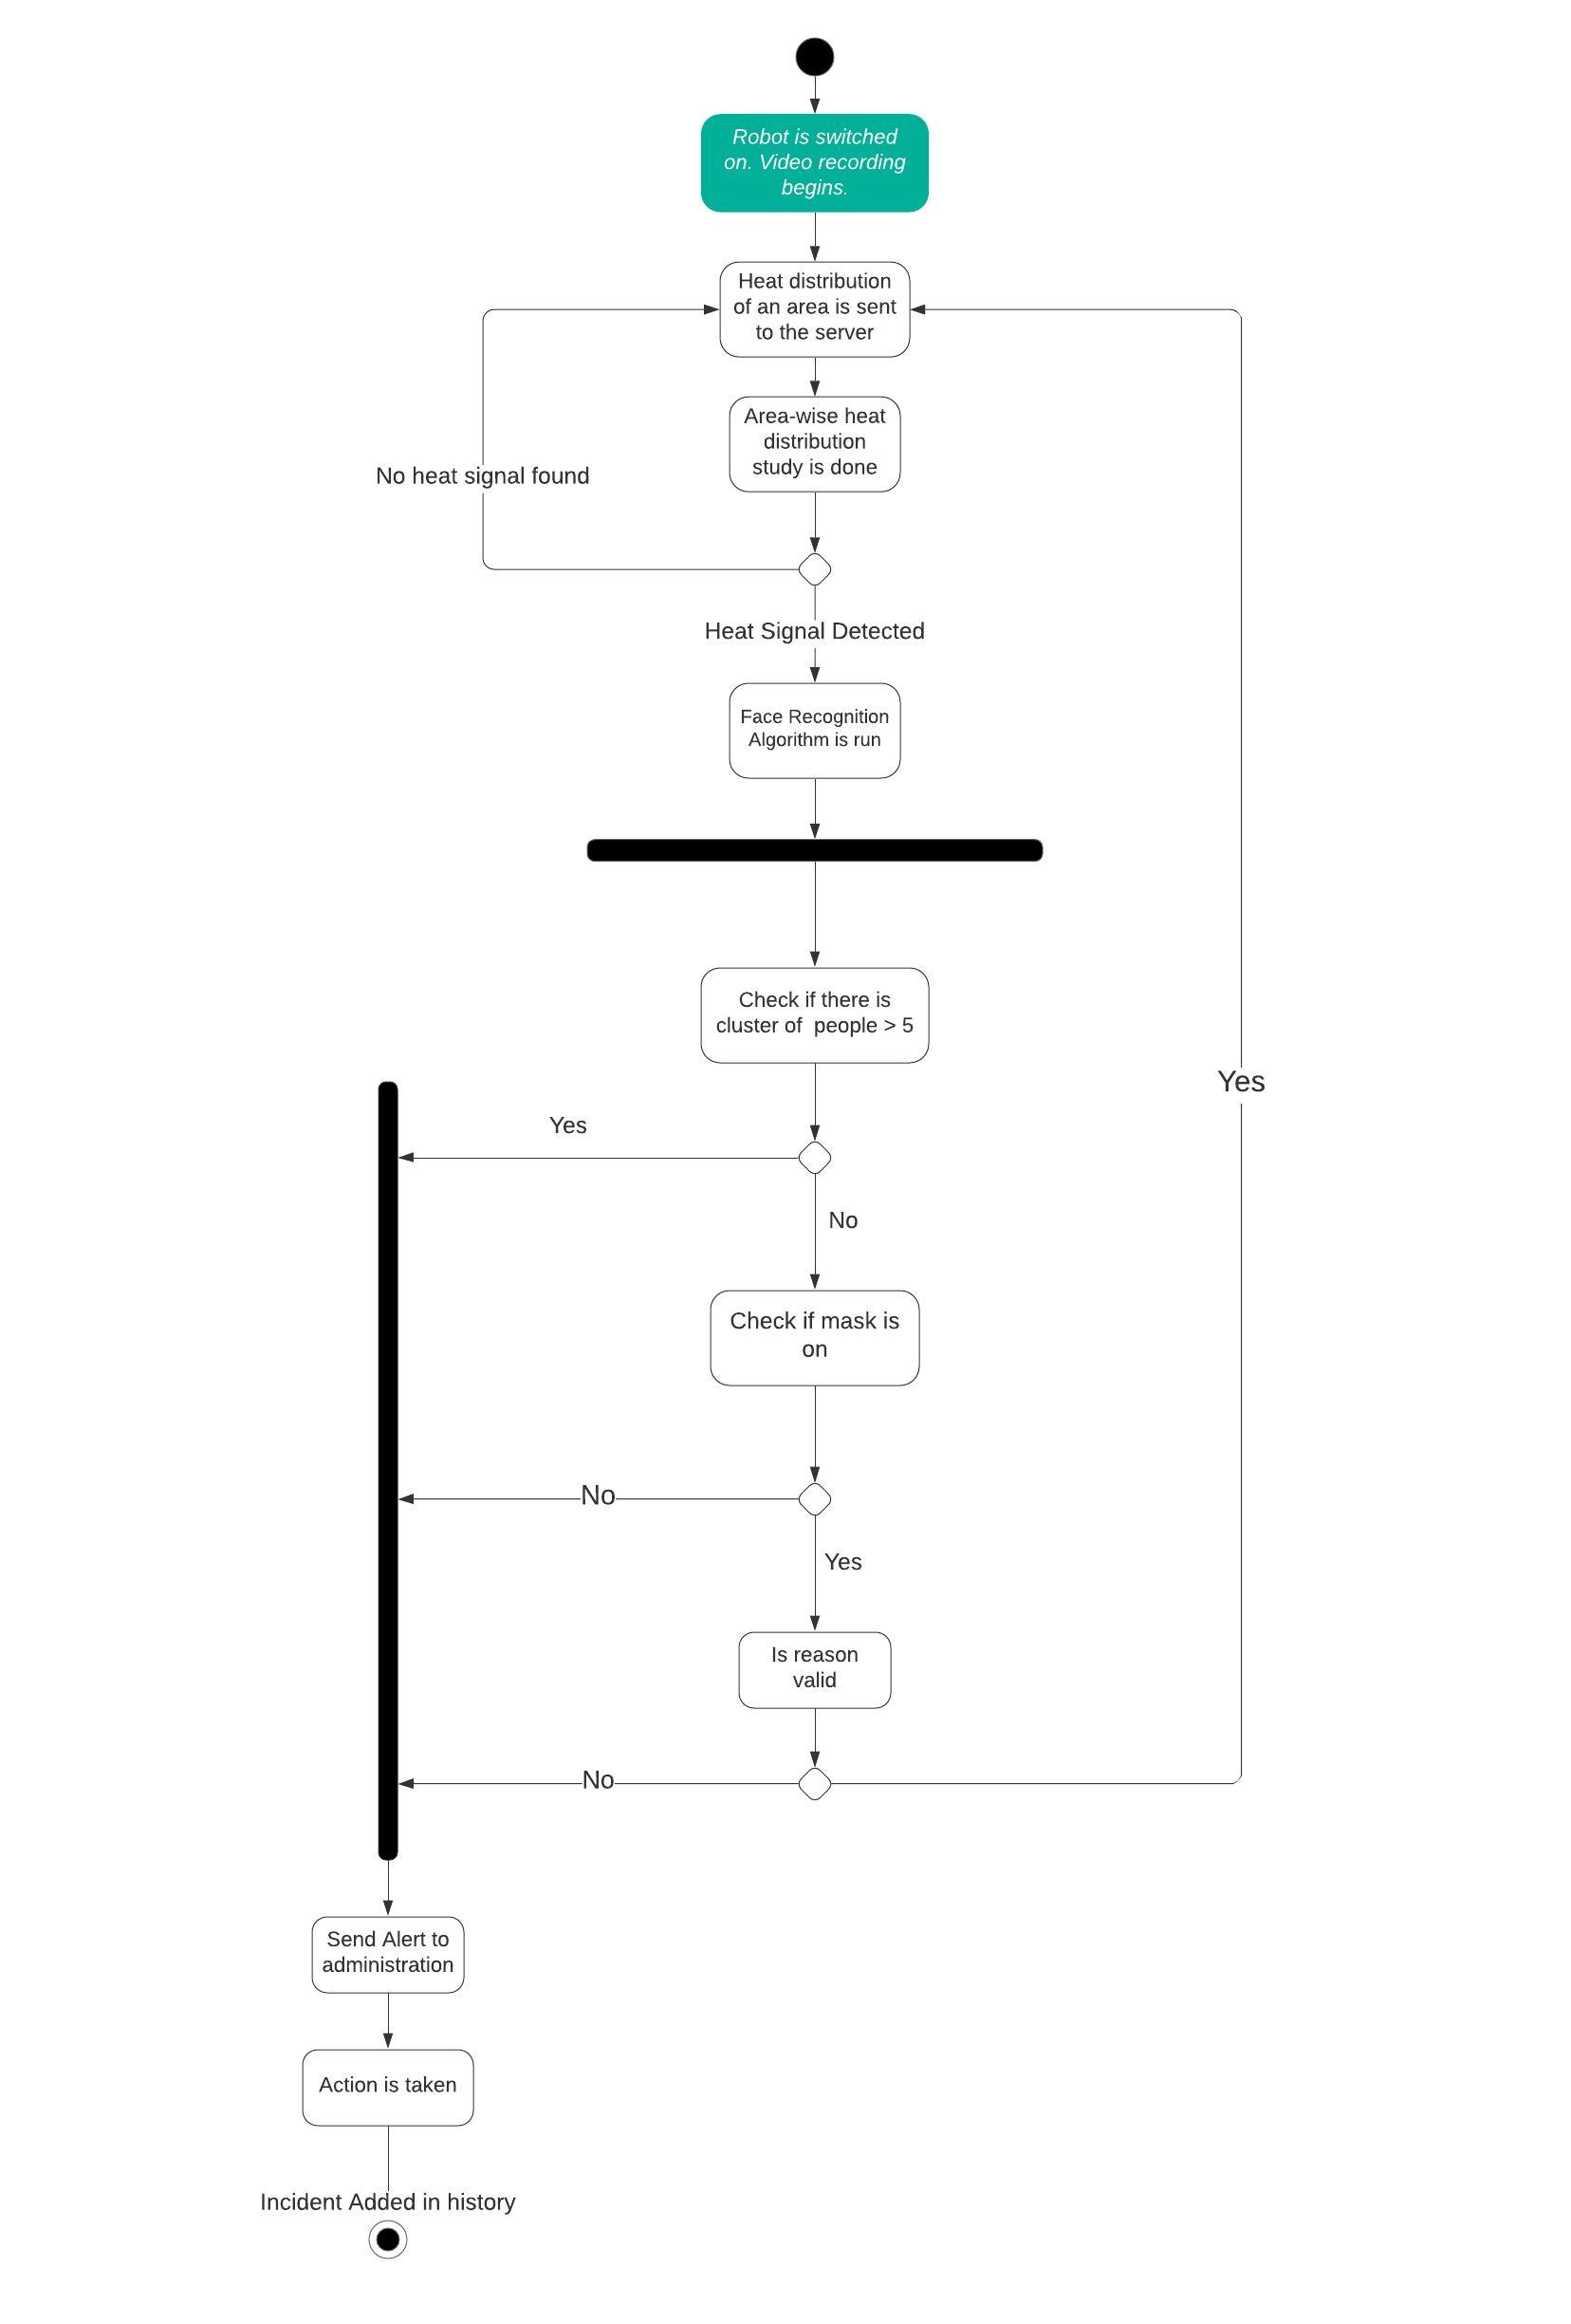
\includegraphics[scale=0.4]{filesFCEFyN-class/state_diagr.jpeg} 
 \caption{State Diagram} \label{fig-2}
 \FloatBarrier
\end{figure}



\section{4. Conclusion}

The proposed solution tries to implement lockdown in a much better way and makes this process more systematic. The machines can be further utilized to implement features like delivery and sanitation. This remains out of the scope for now but can be modified in the future for further development. 

\vspace{4cm}
% Incluir apéndices (si fuera necesario)
\appendix

\begin{thebibliography}{9}

\bibitem{YOLO} 
Joseph Redmon, Santosh Divvala, Ross Girshick and Ali Farhadi
\textit{You Only Look Once:
Unified, Real-Time Object Detection}. 
May 9, 2016
\href{https://arxiv.org/pdf/1503.03832.pdf}{Link}

\bibitem{FaceDetection} 
Florian Schroff, Dmitry Kalenichenko and James Philbin
\textit{FaceNet: A Unified Embedding for Face Recognition and Clustering}. 
June 17, 2015
\href{https://arxiv.org/pdf/1503.03832.pdf}{Link}



\bibitem{Modified YOLO}
Zhao, Xia and Ni, Yingting and Jia, Haihang.
\textit{Modified Object Detection Method Based on YOLO.} 

\href{https://www.sciencedirect.com/science/article/pii/S1110016818301091#!}{Link}


\bibitem{CCTV}
Saleem Almaqashi
\textit{GPS and CCTV Based Security Monitoring System for the Security of School Children}

\href{https://www.researchgate.net/publication/334730218_GPS_and_CCTV_Based_Security_Monitoring_System_for_the_Security_of_School_Children}{Link}

\bibitem{IIITH}
Sarita Chebbi
\textit{When Your Campus Is A Rakshak}

\href{https://blogs.iiit.ac.in/gocoronago/}{Link}

\bibitem{Diplomat}
Reuters,Sankalp Phartiyal, Alasdair Pal
\textit{India’s daily COVID-19 cases pass 400,000 for first time as second wave worsens}

\href{https://www.reuters.com/world/asia-pacific/india-posts-record-daily-rise-covid-19-cases-401993-2021-05-01/}{Link}

\bibitem{Change}
 Kaunain Sheriff M 
\textit{What has changed in the second wave of Covid-19?}

\href{https://indianexpress.com/article/explained/explained-whats-changed-in-second-wave-7289002/}{Link}

\bibitem{Scroll}
Vijayta Lalwani
\textit{How is India’s second wave of Covid-19 different from the first?}

\href{https://scroll.in/article/992165/are-younger-people-at-greater-risk-in-indias-second-wave-of-covid-19}{Link}

\bibitem{WHO}
Joint statement by ILO, FAO, IFAD and WHO
\textit{Impact of COVID-19 on people's livelihoods, their health and our food systems}

\href{https://www.who.int/news/item/13-10-2020-impact-of-covid-19-on-people's-livelihoods-their-health-and-our-food-systems}{Link}

\bibitem{MRC}
Reza Bahmanyar, Eleonora Vig, Peter Reinartz
\textit{MRCNet: Crowd Counting and Density Map Estimation in Aerial and Ground Imagery}

\href{https://arxiv.org/pdf/1909.12743.pdf}{Link}

\bibitem{SSDM}
Reza Bahmanyar, Eleonora Vig, Peter Reinartz
\textit{A real time DNN-based face mask detection system using single shot multibox detector and MobileNetV2}

\href{https://www.ncbi.nlm.nih.gov/pmc/articles/PMC7775036/}{Link}

\bibitem{Smart}
Hameed Khan, K. K. Kushwah, Saurabh Singh, Harshika Urkude
\textit{Smart technologies driven approaches to tackle COVID-19 pandemic: a review}

\href{https://www.ncbi.nlm.nih.gov/pmc/articles/PMC7799428/}{Link}

\bibitem{Facenet}
Florian Schroff, Dmitry Kalenichenko, James Philbin
\textit{FaceNet: A Unified Embedding for Face Recognition and Clustering}

\href{https://arxiv.org/abs/1503.03832/}{Link}


\end{thebibliography}



\end{document}
